\section{Introduction} \label{sec:intro}
A powerful tool for modeling the complexity of the physical world is to frame this complexity as the composition of simpler entities and processes.
For example, the study of classical mechanics in terms of macroscopic objects and a small set of laws governing their motion has enabled not only an explanation of natural phenomena like apples falling from trees but the invention of structures that never before existed in human history, such as skyscrapers.
Paradoxically, the creative \textit{variation} of such physical constructions in human society is due in part to the \textit{uniformity} with which human models of physical laws apply to the literal building blocks that comprise such structures -- the reuse of the same simpler models that apply to primitive entities and their relations in different ways obviates the need, and cost, of designing custom solutions from scratch for each construction instance.

The challenge of scaling the generalization abilities of learning robots follows a similar characteristic to the challenges of modeling physical phenomena: the complexity of the task space may scale combinatorially with the configurations and number of objects, but if all scene instances share the same set of objects that follow the same physical laws, then transforming the problem of modeling scenes into a problem of modeling objects and the local physical processes that govern their interactions may provide a significant benefit in generalizing to solving novel physical tasks the learner has not encountered before. This is the central hypothesis of this paper. 

We test this hypothesis by defining models for perceiving and predicting raw observations that are themselves compositions of simpler functions that operate locally on \textit{entities} rather than globally on scenes.
Importantly, the symmetry that all objects follow the same physical laws enables us to define these learnable entity-centric functions to take as input argument a variable that represents a generic entity, the specific instantiations of which are all processed by the same function.
We use the term \textit{entity abstraction} to refer to the abstraction barrier that isolates the abstract \textit{variable}, which the entity-centric function is defined with respect to, from its concrete \textit{instantiation}, which contains information about the appearance and dynamics of an object that modulates the function's behavior.

\begin{figure}[!t]
\centering
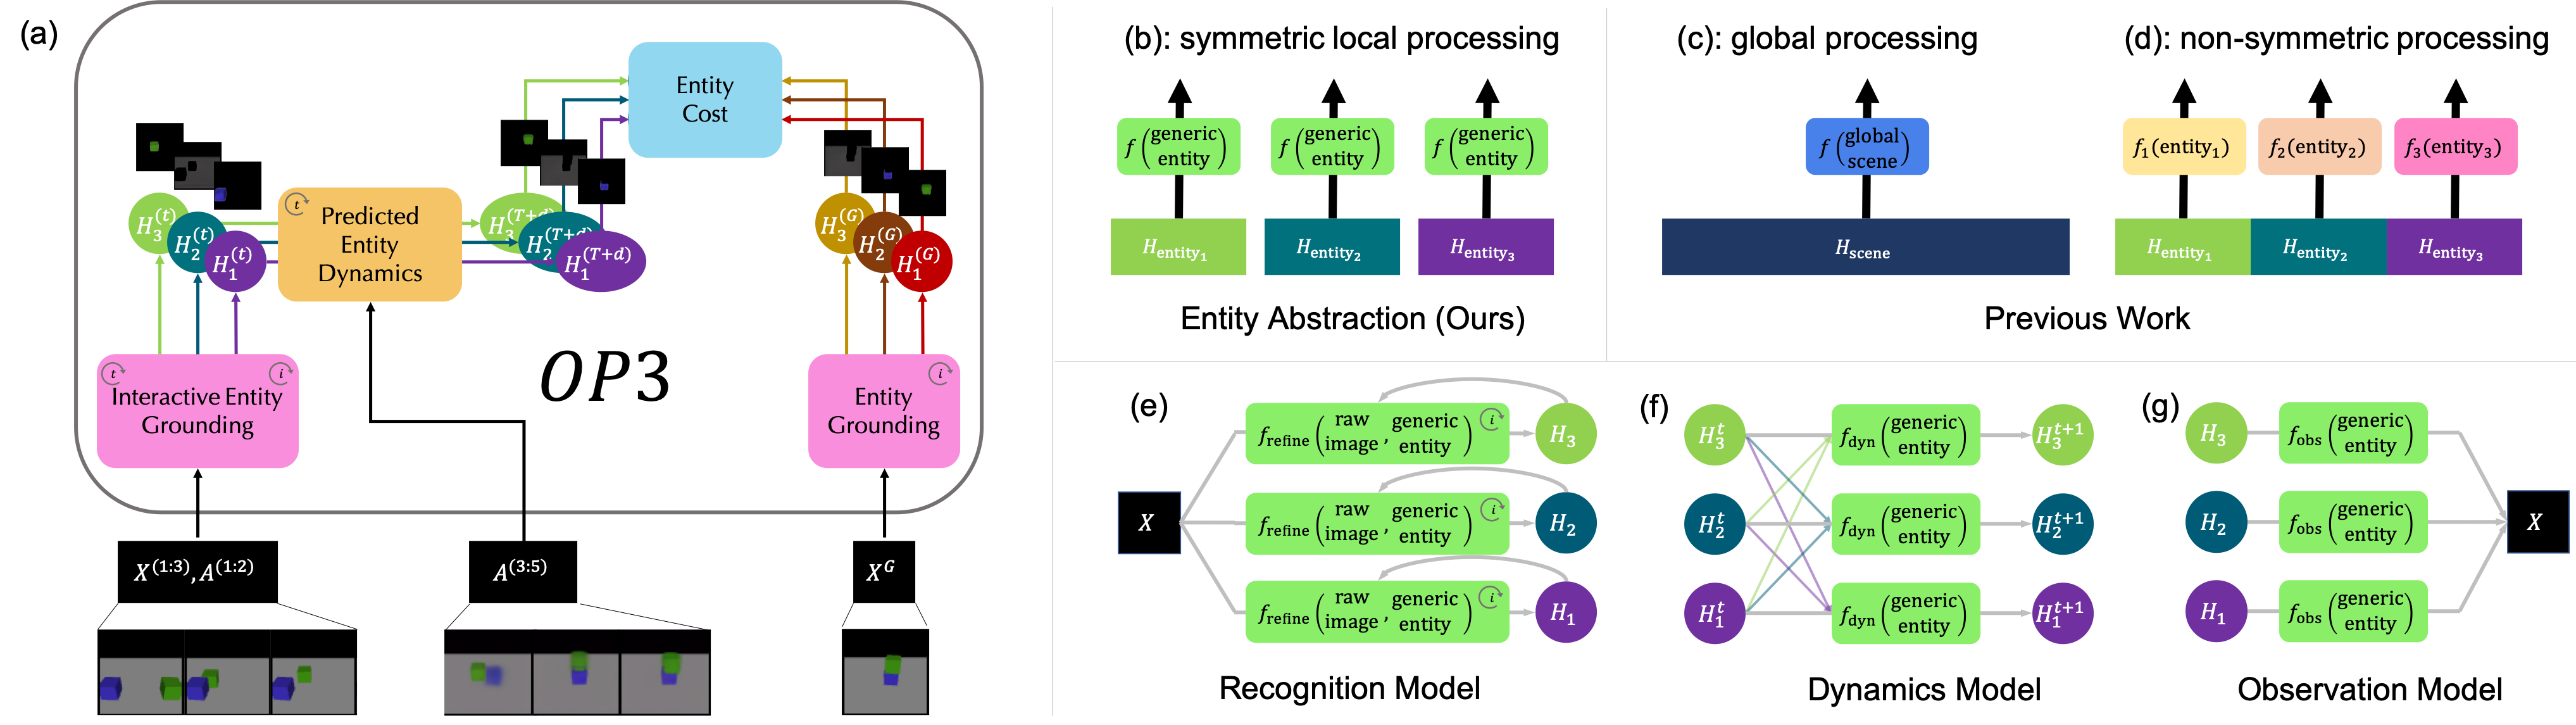
\includegraphics[width=0.95\textwidth]{figs/method/combined_overview.png}
\caption{\small{
\textbf{OP3}. \textbf{(a)} OP3 can infer a set of entity variables $H^{(T)}_{1:K}$ from a series of interactions (interactive entity grounding) or a single image (entity grounding). OP3 rollouts predict the future entity states $H^{(T+d)}_{1:K}$ given a sequence of actions $a^{(T:T+d)}$. We evaluate these rollouts during planning by scoring these predictions against inferred goal entity-states $H^{(G)}_k$.
\textbf{(b)} OP3 enforces the \textbf{entity abstraction}, factorizing the latent state into \textit{local} entity states, each of which are symmetrically processed with the same function that takes in a \textit{generic entity} as an argument.
In contrast, prior work either \textbf{(c)} process a global latent state~\citep{hafner2018learning} or \textbf{(d)} assume a fixed set of entities processed in a permutation-sensitive manner~\citep{finn2016unsupervised,kulkarni2019unsupervised,xu2018modeling,watters2019cobra}.
\textbf{(e-g)} Enforcing the entity-abstraction on modeling the \textbf{(f)} dynamics and \textbf{(g)} observation distributions of a POMDP, and on the \textbf{(e)} \textbf{interactive inference} procedure for grounding the entity variables in raw visual observations. Actions are not shown to reduce clutter.
}}
\label{fig:combined_overview}
\vspace{-10pt}
\end{figure}

Defining the observation and dynamic models of a model-based reinforcement learner as neural network functions of abstract entity variables allows for symbolic computation in the space of entities, but the key challenge for realizing this is to ground the values of these variables in the world from raw visual observations.
Fortunately, the language of partially observable Markov decision processes (POMDP) enables us to represent these entity variables as latent random state variables in a state-factorized POMDP, thereby transforming the variable binding problem into an inference problem with which we can build upon state-of-the-art techniques in amortized iterative variational inference~\citep{marino2018iterative,marino2018general,greff2019iodine} to use temporal continuity and interactive feedback to infer the posterior distribution of the entity variables given a sequence of observations and actions.

We present a framework for \textit{object-centric perception, prediction, and planning} (OP3), a model-based reinforcement learner that predicts and plans over entity variables inferred via an \textit{interactive inference} algorithm from raw visual observations.
Empirically OP3 learns to discover and bind information about actual objects in the environment to these entity variables \textit{without any supervision on what these variables should correspond to.}
As all computation within the entity-centric function is \textit{local in scope} with respect to its input entity, the process of modeling the dynamics or appearance of each object is \textit{protected} from the computations involved in modeling other objects, which allows OP3 to generalize to modeling a variable number of objects in a variety of contexts with no re-training.

\textbf{Contributions:} 
Our conceptual contribution is the use of entity abstraction to integrate graphical models, symbolic computation, and neural networks in a model-based reinforcement learning (RL) agent.
This is enabled by our technical contribution: defining models as the composition of locally-scoped entity-centric functions and the interactive inference algorithm for grounding the abstract entity variables in raw visual observations without any supervision on object identity.
Empirically, we find that OP3 achieves two to three times greater accuracy than state of the art video prediction models in solving novel single and multi-step block stacking tasks.